\documentclass[11pt]{article}
\setlength{\textwidth}{6.5in}
\setlength{\oddsidemargin}{0pt}
\setlength{\evensidemargin}{0pt}
\setlength{\textheight}{9in}
\setlength{\topmargin}{0pt}
\addtolength{\topmargin}{-\headheight}
\addtolength{\topmargin}{-\headsep}
\ifdefined\pdfpagewidth \pdfpagewidth=8.5in \pdfpageheight=11in \fi
\ifdefined\pagewidth \pagewidth=8.5in \pageheight=11in \fi
\usepackage{pgfplots}
\usepgfplotslibrary{groupplots}
\pgfplotsset{compat=1.16, stq/.style={scale only axis, width=3.85cm,
  height=3.5cm, every axis plot/.append style={black, thin}, mark size=1.5pt,
  mark options={solid}, tick label style={font=\scriptsize},
  label style={font=\footnotesize}, title style={font=\footnotesize},
  legend style={font=\scriptsize, draw=none, fill=none},
  legend cell align=left, xminorticks=false}}

\newcommand{\code}[1]{\texttt{#1}}
\emergencystretch=3em
\newcommand{\sqg}{\sqrt{g}}
\newcommand{\cellA}[1]{\parbox[t]{3.3cm}{\raggedright\strut#1\strut}}
\newcommand{\cellB}[1]{\parbox[t]{4.0cm}{\raggedright\strut#1\strut}}
\newcommand{\cellC}[1]{\parbox[t]{4.6cm}{\raggedright\strut#1\strut}}
\newcommand{\cellD}[1]{\parbox[t]{3.0cm}{\raggedright\strut\scriptsize#1\strut}}
\newtheorem{theorem}{Theorem}
\makeatletter
\def\sq@slash{/}
\newcommand{\link}[1]{\texttt{\@tfor\sq@t:=#1\do{\sq@t\ifx\sq@t\sq@slash\allowbreak\fi}}}
\makeatother

\title{Stellarocq: Machine-Checked Certificates for Stellarator Equilibria}
\author{Charles C. Norton\\\normalsize\texttt{cnorton2@binghamton.edu}}
\date{}

\begin{document}
\maketitle

\begin{abstract}
VMEC judges its output by its own convergence metric, which measures the
retained Fourier harmonics of its forces and not the field reconstructed from
its output file. Stellarocq states properties of that field as machine-checked
theorems. A Rocq development reconstructs the field from the exact numbers of a
VMEC++ output file and proves that the residual it evaluates at a free radius is
the field's ideal-MHD force; on the grid's surfaces it evaluates VMEC's discrete
form of that force. Bounds, Fourier harmonics, flux-surface integrals, the
Mercier criterion and the existence of discrete solutions are decided by
checkers extracted from their soundness proofs. On manufactured problems the
certified error of the collocated half-grid rule, known to twelve digits, falls
about fourfold per doubling of the surfaces. On VMEC++ equilibria the
certificates show a resonant force harmonic falling only 1.2 to 1.4-fold per
doubling, a free-boundary pressure jump that refinement barely reduces, a
Mercier criterion whose sign at coarse resolution depends on the radial
differencing, and a W7-X force set by the Fourier truncation. The development
also proves that Landreman's explicit three-dimensional fields, counterexamples
to Grad's conjecture, are ideal-MHD equilibria; VMEC++ converges to a member of
one of his families at about second order and does not converge to a member of
the other.
\end{abstract}

\section{Introduction}

The Variational Moments Equilibrium Code (VMEC)~\cite{hirshman1983,hirshman1986}
computes three-dimensional ideal-MHD equilibria with nested flux surfaces by
minimizing the plasma energy over Fourier representations of the surfaces. It
and its reimplementation VMEC++~\cite{schilling2025,vmecpp} sit at the centre of
stellarator design and optimization. A run ends with a \emph{wout} file: Fourier
coefficients of the surfaces on a radial grid, profiles, and derived quantities
such as the Mercier stability terms, all in binary64 floating point.

What such a file establishes about the field it describes is judged by
convergence metrics internal to the solver and by diagnostics recomputed in
floating point, and those judgements can mislead in ways the file does not
show. The normalized force residual a run drives below $10^{-12}$ concerns the
Fourier harmonics of the forces the solver balances, while the force of the
field reconstructed from the file, at points of its surfaces, can be set by the
angular truncation and not fall as the radial grid is refined. A Mercier term
computed from radial differences of the file's profiles can change sign when
the differences are taken another way. A rational surface can carry a current
sheet that the solution resolves more slowly than anything else as the radial
grid is refined. Each of these is a statement about the reconstructed field,
and each can be decided exactly.

Stellarocq decides them as theorems. The object of every statement is the field
reconstructed from the exact numbers in the file by the solver's own rule
between nodes and half points, extended to every radius by cubic Hermite
interpolation. A claim about that field, such as a
bound on its force at a set of points, is decided by a checking function: a
program written in the Rocq proof assistant~\cite{rocq}, proven once for all
inputs to imply the claim whenever it returns \code{true}, and extracted to
OCaml~\cite{letouzey2003} to run as compiled code. The checking functions
compute in interval arithmetic, whose results contain the exact values however
the floating-point rounding falls, with real-number semantics and intervals
from Coquelicot~\cite{coquelicot}, Flocq~\cite{flocq} and
CoqInterval~\cite{melquiond2008}. A certificate carries the file's numbers and
the claimed bounds, so anyone can check it again with the released checker
without trusting the program that wrote it.

Section~\ref{sec:object} defines the reconstructed field, proves that the
residual Stellarocq evaluates at a free radius is its ideal-MHD force, and gives
exactly how its
Jacobian and metric differ from the ones VMEC forms. Section~\ref{sec:certs}
describes the checking functions, for bounds at points and over cells, discrete
Fourier harmonics, flux-surface integrals, the Mercier criterion and the
existence of discrete solutions, and how the development that proves them is
built. Section~\ref{sec:results} applies them to VMEC++ and to Landreman's
explicit three-dimensional fields~\cite{landreman2026}, counterexamples to
Grad's conjecture both of whose families the development proves to be ideal-MHD
equilibria, so that a solver's distance from them is a true error.

The certificates make such effects proven numbers about the reconstructed field.
On manufactured problems the certified error of the collocated half-grid rule,
known to twelve digits, falls about fourfold per doubling of the surfaces. On a
rational surface the resonant harmonic of the force falls only 1.2 to 1.4-fold
per doubling of the surfaces, while the axisymmetric harmonics fall fourfold. At
the free boundary the pressure jump falls by factors of only 1.05 to 1.14 per
doubling of the surfaces, for every vacuum field between the answers of two
independent solvers. On W7-X, converged to $f_{sqr}<10^{-12}$, the certified
bound on the force at points of its surfaces does not fall as the surfaces
double and falls as the angular resolution rises. At coarse resolution the certified
Mercier criterion takes either sign, depending on how the radial derivatives are
taken. VMEC++ converges at about second order to Landreman's sheared
equilibrium away from the axis and does not converge to his equilibrium with
$\iota=2$. Section~\ref{sec:users} draws the consequences for users of VMEC,
and the tests these results added to VMEC++ close Section~\ref{sec:results}.

\section{The certified object}\label{sec:object}

A wout file holds Fourier coefficients on a radial grid, not a field.
Stellarocq defines the field by the solver's own rule between nodes and half
points, extends it to every radius by a cubic Hermite interpolation of its own
choosing, and computes the field and the force of ideal MHD exactly from the
coordinates that result.

\paragraph{Reconstruction.}
VMEC keeps the surface coefficients of $R$ and $Z$ on the full radial grid
$s_j = jh$ and the stream function $\lambda$, the rotational transform $\iota$
and every field quantity on the half grid $s_{j+1/2}$. Stellarocq's
\code{Physics.v} writes the rule that connects them. On a half point $s_h$
between nodes $a$ and $b$, a coefficient of even poloidal mode number is the
mean of its two node values and one of odd mode number is averaged with the
$\sqrt{s}$ weight VMEC folds into its Jacobian,
\begin{equation}
c_k(s_h) = {\textstyle\frac12}\bigl(c_k(a)+c_k(b)\bigr)\ \ (m_k \mbox{ even}),\qquad
c_k(s_h) = {\textstyle\frac12}\sqrt{s_h}\,\Bigl(\frac{c_k(a)}{\sqrt{s_a}}+\frac{c_k(b)}{\sqrt{s_b}}\Bigr)\ \ (m_k \mbox{ odd}),
\end{equation}
with radial derivatives the matching difference quotients and angular
derivatives exact derivatives of the series $R=\sum_k c_k\cos(m_k u-n_k v)$,
$Z=\sum_k z_k\sin(m_k u-n_k v)$. The half-grid $\lambda$ and $\iota$ are the
file's own, $\Phi'$ is constant, and the pressure is the input's profile. For
statements at an arbitrary radius each coefficient of $R$ and $Z$ is the cubic
Hermite interpolant of its half-point values and slopes, which agrees with the
half-grid rule at the half points; $\lambda$ follows the same parity rule
linearly between half points, and $\iota$ is linear there.

\paragraph{Field and residual.}
With $\sqg = R(R_uZ_s-R_sZ_u)$, the field is
$B^u=\Phi'(\iota-\lambda_v)/\sqg$, $B^v=\Phi'(1+\lambda_u)/\sqg$, its covariant
components are $B_i=g_{iu}B^u+g_{iv}B^v$, and
$\mu_0\sqg J^s=\partial_uB_v-\partial_vB_u$. The residual of
$\mathbf{J}\times\mathbf{B}=\nabla p$ has the components
\begin{equation}
r_u = -\mu_0\sqg J^s B^v,\qquad r_v = \mu_0\sqg J^s B^u,\qquad
r_s = (\partial_vB_s-\partial_sB_v)B^v-(\partial_sB_u-\partial_uB_s)B^u-\mu_0\,\frac{dp}{ds},
\end{equation}
written in \code{Physics.v} as trees of a deep expression language. Read at a
free radius, with every radial derivative that of the Hermite reconstruction,
they form the continuum residual. Let $X(s,u,v)=(R\cos v,R\sin v,Z)$ be the
reconstructed coordinate map, $\mathbf{e}_s$, $\mathbf{e}_u$ and $\mathbf{e}_v$
its partial derivatives, and $\mathbf{B}=B^u\mathbf{e}_u+B^v\mathbf{e}_v$ the
reconstructed field as a function of $(s,u,v)$.

\begin{theorem}[\code{continuum\_force\_coords}]
Let the slots of the residual's expressions hold a state's radii, coefficients,
flux, transform and pressure derivative $p'$, and let $(s_0,u_0,v_0)$ be a point
where $\sqg\neq0$. There let $\nabla s=\mathbf{e}_u\times\mathbf{e}_v/\sqg$,
$\nabla u=\mathbf{e}_v\times\mathbf{e}_s/\sqg$ and
$\nabla v=\mathbf{e}_s\times\mathbf{e}_u/\sqg$, and let $\partial_s\mathbf{B}$,
$\partial_u\mathbf{B}$ and $\partial_v\mathbf{B}$ be the derivatives of
$\mathbf{B}$ along the three coordinate lines through the point. Then the three
outputs of the continuum residual there are $\mathbf{F}\cdot\mathbf{e}_s$,
$\mathbf{F}\cdot\mathbf{e}_u$ and $\mathbf{F}\cdot\mathbf{e}_v$, with
\begin{equation}
\mathbf{F}=\bigl(\nabla s\times\partial_s\mathbf{B}+\nabla u\times\partial_u\mathbf{B}
+\nabla v\times\partial_v\mathbf{B}\bigr)\times\mathbf{B}-\mu_0p'\,\nabla s.
\end{equation}
\end{theorem}

\noindent In words, the three outputs are the covariant components of
$\mu_0(\mathbf{J}\times\mathbf{B}-\nabla p)$ for the reconstructed field, with
$\nabla p=p'\nabla s$: the bracket is the curl of $\mathbf{B}$ in the
coordinates $x^j=s,u,v$, since the Cartesian derivative of $\mathbf{B}$ is
$\sum_j\nabla x^j\otimes\partial_j\mathbf{B}$, and every quantity in the
statement is a formula in the reconstruction's derivatives at the point.
\code{continuum\_force} gives the same outputs through the Cartesian curl: for
any $\mathbf{G}:\mathbf{R}^3\to\mathbf{R}^3$ and $P:\mathbf{R}^3\to\mathbf{R}$
differentiable at $X(s_0,u_0,v_0)$ and equal to the reconstructed field and
pressure along the three coordinate lines through it, they are
$\mathbf{F}\cdot\mathbf{e}_i$ with
$\mathbf{F}=(\nabla\times\mathbf{G})\times\mathbf{G}-\mu_0\nabla P$.
\code{continuum\_force\_asym\_coords} and \code{continuum\_force\_asym} are the
two statements for a state without stellarator symmetry, and they rest on the
identities at one point \code{Force.force\_coords} and \code{Force.force\_law}.

At a node the solver's rule is used instead. The angular outputs are the
formulas above at the outer half point, and the radial output is VMEC's
combination of the fields at the two half points, with centred differences for
radial derivatives; each of those fields is that of the series with VMEC's
half-grid values and slopes (\code{node\_residual}, \code{node\_residual\_asym}).

\paragraph{VMEC's products.}
Every half-point quantity that is linear in the coefficients, $R$, $Z$ and their
derivatives, agrees with VMEC's term for term. The Jacobian and the metric
elements are products, which VMEC forms from averages over the two nodes of
products of node values, where the reconstruction multiplies the interpolated
series. \code{VmecKernel.v} transcribes VMEC++'s kernels and proves the
differences exactly. With $r$, $z$ the even parts and $\hat r$, $\hat z$ the odd
parts divided by $\sqrt{s}$ of the node values, and $\Delta$ the outer node's
value less the inner one's, the reconstruction's factor $R_uZ_s-R_sZ_u$ and
VMEC's $\tau$ satisfy
\begin{equation}
(R_uZ_s-R_sZ_u)-\tau=-{\textstyle\frac18}\bigl(\Delta\hat r_u\,\Delta\hat z-\Delta\hat z_u\,\Delta\hat r\bigr)
-\frac{1}{8\sqrt{s_h}}\bigl(\Delta r_u\,\Delta\hat z-\Delta z_u\,\Delta\hat r\bigr)
\end{equation}
(\code{vmec\_jacobian\_difference}), and each of $g_{uu}$, $g_{uv}$ and $g_{vv}$
differs from VMEC's by a sum of such products (\code{vmec\_metric\_difference}).
Where every node difference in the identity is at most $K|h|$, the two
Jacobian factors agree to within ${\textstyle\frac14}(Kh)^2(1+s_h^{-1/2})$
(\code{vmec\_jacobian\_second\_order}). The certified field is the
reconstruction's, and VMEC's discrete field differs from it by these terms,
of second order in the radial step away from the axis. Evaluated in floating point
(\code{gen/jacobian\_gap.py}) on the stellarator-symmetric files of
Section~\ref{sec:results}, the two Jacobians, and so the two $\sqg$
(\code{vmec\_sqrtg\_difference}), differ by at most a relative
$8.9\times10^{-5}$ on the half-grid surfaces whose nodes lie off the axis, the
largest on W7-X at 49 surfaces near the axis. On the surfaces with $s\ge1/4$
the difference falls as the surfaces double, on W7-X from $2.3\times10^{-5}$ at
49 surfaces to $1.5\times10^{-6}$ at 193 and on Landreman's sheared equilibrium
from $6.3\times10^{-7}$ at 13 to $1.2\times10^{-9}$ at 200.

\paragraph{Identities.}
The representation builds some properties in, and for the reconstruction they
are theorems: it is solenoidal
(\code{divergence\_free}), the $(0,0)$ coefficient of $\lambda$ drives nothing
(\code{lambda\_gauge}), which exhibits the poloidal relabelling as an exact
kernel direction, and the residual has no component along the field
(\code{residual\_along\_field}). The
Euler--Lagrange expressions of VMEC's energy $W=\int(B^2/2-\mu_0p)\sqg$ at fixed
$\lambda$, $\iota$, flux and pressure are $-\sqg$ times the cylindrical
components of the force (\code{energy\_gradient\_is\_force}), so that the
forces the solver drives to zero are the ideal-MHD force. \code{Hypotheses.v}
states the physical premises some theorems carry, such as nested flux surfaces
and a scalar pressure.

\section{Certificates and their soundness}\label{sec:certs}

A certificate is a text file that a generator in \code{gen/} writes from a wout
file. It carries every number of the file it uses as an integer mantissa and a
power-of-two exponent, so no rounding happens between the file and the
certificate, together with the bounds it claims. The extracted checker
recomputes every enclosure from those numbers, and no bound the generator
computes is trusted. A check passes when its enclosures, intervals that contain
the exact values, lie inside the claimed bounds, and its soundness theorem turns
that comparison into a theorem about the field.

\paragraph{Expressions and intervals.}
\code{Expr.v} gives an expression two meanings: a value over extended reals, in
which division by zero and the square root of a negative number give
\code{Xnan}, and a value over CoqInterval's floating-point intervals.
\code{ieval\_correct} states that the interval contains the extended-real value,
so a bounded output interval proves both that the value is a real number and
that it lies in the bounds. Because the embedding is deep, one tree carries both
meanings. \code{Deriv.v} differentiates it symbolically with a chain rule proven
in the extended-real sense, and subexpressions that the residual's components
share are bound once to environment slots.

\paragraph{Points and cells.}
A point certificate bounds the residual at points (\code{check\_cert\_correct}).
A cell certificate bounds a component over a rectangle of two varied slots, two
angles or an angle and the radius, by its value at the centre plus enclosures of
its derivatives over the rectangle times the half-widths
(\code{check\_ccert\_correct}); reversed, the same data bounds a component away
from zero. The bound tightens as the cells shrink, since each derivative
enclosure is taken over its own cell. On one surface of the Solov'ev
equilibrium, where the residual reaches $4.1\times10^{-7}$ in floating point,
the bound falls from $2.2\times10^3$ with 8 cells to $7.7\times10^{-6}$ with
8192, about sixteen-fold per fourfold refinement from 128 cells on.
\code{Cover2.v} decides, column by column, that the cells of a verdict cover the
rectangle they span (\code{cells\_cover\_rect}) or every line they lie on
(\code{cells\_cover\_lines}).

\paragraph{Harmonics and integrals.}
A spectral solver balances forces mode by mode: VMEC drives to zero the
harmonics, at the modes it retains, of $\sqg$ times the cylindrical components
of the force (\code{energy\_gradient\_is\_force}). \code{Project.v} encloses the
discrete Fourier harmonic of a covariant component of the residual at a
retained mode (\code{harm\_encloses}). That component contracts the force with
a coordinate tangent vector and carries no $\sqg$ weight, so its harmonic at a
retained mode also carries the modes VMEC drops and need not vanish when VMEC's
do. \code{Harmonic.v} integrates
exactly the components whose trigonometric degree lies below an equispaced
grid's point counts. \code{Integrate.v} encloses other flux-surface integrals by
the midpoint rule over a lattice of cells that the checker lays out itself, with
the error read off its own enclosures of the second derivatives over each cell
(\code{integ2\_correct}, \code{integ1\_correct}). \code{MercierRun.v} assembles
DShear, DCurr, DWell, DGeod and DMerc as VMEC's \code{mercier.f90} defines
them~\cite{mercier1960,bauer1984} from integrals over the whole angular torus
that the same run computes. Its lattice reaches past each period of $2\pi$,
which ends inside the last cells, and the two strips it adds there are bounded
through the integrand's enclosures over those cells
(\code{integ2\_torus\_correct}), so a verdict is a theorem about the criterion
of the reconstruction (\code{merc\_run\_correct}).

\paragraph{Boxes of states.}
In \code{Box.v} every input slot carries a half-width, so one evaluation covers
every field whose coefficients lie in a box. The theorem behind the resonant
harmonic of Section~\ref{sec:results} shows the form every soundness theorem
takes:
\begin{verbatim}
Theorem dharm_correct :
  forall c, check_dharm c = true ->
  forall xs, in_box (hc_ms c) (hc_ds c) xs ->
  contains (I.convert (harm_total c))
           (Xreal (dsum2 (hc_Nu c) (hc_Nv c) 0 0 (harm_fun c xs))).
\end{verbatim}
For a certificate \code{c} whose check passes and every state \code{xs} in its
box, the equispaced sum of the component times the harmonic's kernel over the
certificate's grid of angles is a real number, and it lies in the interval
\code{harm\_total c} that the same computation returns.

\paragraph{Discrete equilibria.}
\code{Newton.v} proves that a passing interval Newton test in Krawczyk
form~\cite{krawczyk1969,moore2009} on any system of expressions gives exactly one
zero in its box: $x-AF(x)$ maps the box into itself as a contraction, and an
approximate inverse $A$ makes its fixed point a zero of $F$. \code{Colloc.v}
collocates the residual over a band of surfaces as such a system, with the
surface coefficients as unknowns (\code{colloc\_correct}). \code{Wide.v}
evaluates the system's outputs at the centre of the box in floating point of
any precision.

\paragraph{Proof engineering.}
The theorems and checkers of this paper rest on 39 files and about 27\,000 lines
of Rocq with about 800 theorems and lemmas, part of a development of 167 files
that \code{make all} builds, with the checker, in about four minutes with six
parallel jobs. Each kind of claim is decided by a Rocq
function on syntax, proven sound once for all inputs, and the kernel never
evaluates a certificate, so no proof term grows with one and a check costs what
compiled OCaml costs. The physics enters only through expression trees, which
\code{Deriv.v} differentiates and every checker evaluates in intervals proven to
contain their one extended-real meaning: binary64 intervals on Rocq's primitive
floats (\code{ieval\_correct}) and, for the checks at 120 to 256 bits,
CoqInterval's floats with integer mantissas of any precision
(\code{weval\_correct}). A theorem about what a tree means thus serves every
certificate that evaluates it.

\paragraph{Trust base.}
The kernel checks the proofs; what runs is the OCaml extraction of the checking
functions, linked with a driver that parses certificates into the extracted data
types, divides the checking among processes and prints verdicts. The trusted
components are the Rocq kernel and extraction, which realizes Rocq's natural
numbers as OCaml's native integers (\code{ExtrOcamlNatInt}), the OCaml
toolchain, the implementation of Rocq's primitive 63-bit integers and binary64
floats, the driver's 3\,900 lines of OCaml with its parser and its division of
the work, and the correspondence between a certificate's numbers and the file
or formulas they are taken from. \code{gen/verify\_cert.py} checks that
correspondence slot by slot against the wout file for the residual, cell,
point, surface and harmonic certificates. The slots no wout holds, the vacuum
pressure of the free-boundary certificates and the parameters of Landreman's
member, stay in the trust base with the data of the Newton certificates. The
classical constructions behind Rocq's real numbers appear only in
specifications, and extraction directives replace them by values that fail
when consulted. The theorems named here rest on the
two axioms of the standard library's classical Dedekind reals, excluded middle,
functional extensionality and the specifications of the primitive operations.
The build pins Rocq 9.1.1 with its
standard library 9.2.0, CoqInterval 4.11.4, Flocq 4.2.2, Coquelicot 3.4.5,
MathComp 2.4.0 and OCaml 4.14.2.

\paragraph{Cost.}
Checking takes seconds to hours (Table~\ref{tab:cost}). A point
certificate evaluates the residual once per point, a cell certificate its
derivatives over each cell and a harmonic every point of its grid, so the cost
grows with the number of modes, the number of points or cells, and the
precision. A harmonic whose rows are evaluated at 256 bits in software floating
point takes hours where the same harmonic in binary64 takes seconds. The
Mercier criterion integrates over the whole torus, and its cells must be narrow
against the highest mode there for the enclosures over them to stay bounded.
Four coverings of 2048 cells take two to three minutes for the tokamak
\code{up\_down\_asym}, while for W7-X, whose toroidal numbers reach 60 on the
torus, a covering of $64\times16$ cells leaves enclosures unbounded. The
checker divides a certificate's points, cells or rows among processes.

\begin{table}[t]
\centering\small
\begin{tabular}{@{}lll@{}}
\hline
Check & Size & Time \\
\hline
points, free-boundary jump & NESTOR's grid & 0.1--3~s \\
points, $\mathbf{B}-\mathbf{B}^*$ of Landreman's field & $64\times32$ points & 3--18~s \\
cells, Solov'ev residual on a surface & 8--8192 cells & up to 15~s \\
cells, free-boundary jump over the boundary & $512\times128$ cells per period & 72 and 78~min \\
harmonic over a box of states, binary64 & $64\times32$ points & 2~s \\
harmonic, rows at 256 bits & $64\times32$ points & 1.4--2.1~h \\
Mercier criterion, tokamak & four coverings of 2048 cells & 2--3~min \\
Newton existence, 120 or 128 bits & up to 423 unknowns & up to 46~min \\
W7-X points and projection & 4096 points, 288--800 modes & 21~min--3.4~h \\
\hline
\end{tabular}
\caption{Time to check each kind of certificate.}\label{tab:cost}
\end{table}

\section{Results}\label{sec:results}

Table~\ref{tab:results} collects the certified results with the theorem each
rests on. The manufactured problems are Stellarocq's collocated systems for the
manufactured mappings of a VMEC++ pull request, still open, that adds a force
source to the solver~\cite{pr784}; every other case is a VMEC++ run or a file
from its test data. The runs of Landreman's equilibrium, of the rippled tokamak
and of W7-X are VMEC++ 0.4.7, and the free-boundary and Mercier runs use the
branch of~\cite{branch}, which reads NESTOR's vacuum field. A number called
certified is one that a passing verdict proves. On the surfaces of a run the
residual is the node rule of Section~\ref{sec:object}, VMEC's discrete form of
the force, which is consistent with the continuum residual to second order away
from the axis (\code{node\_consistent}).

\begin{table}[t]
\centering\footnotesize
\setlength{\tabcolsep}{4pt}
\begin{tabular}{@{}llll@{}}
\hline
\cellA{Case and surfaces} & \cellB{Certified quantity and unit} & \cellC{Values, surface by surface} & \cellD{\footnotesize Theorem} \\
\hline
\cellA{manufactured, 3D; 9, 17, 33, 65} & \cellB{$\max|x_h-x^*|$, $10^{-7}$} & \cellC{27.34, 7.169, 1.830, 0.4607} & \cellD{\code{colloc\_correct}} \\
\cellA{asymmetric; 9, 17, 33} & \cellB{the same, $10^{-6}$} & \cellC{26.91, 7.207, 1.863} & \cellD{\code{colloc\_correct}} \\
\cellA{Solov'ev; 1, 2, 3} & \cellB{zero of the collocated residual} & \cellC{one in each box, radius $6.0\times10^{-10}$ to $7.7\times10^{-9}$} & \cellD{\code{colloc\_correct}} \\[2pt]
\cellA{rippled tokamak; 65, 129, 257, 513, 1025} & \cellB{$(2,1)$ harmonic of $r_s$ at $\iota=1/2$, 256 bits, $10^{-5}$~T$^2$} & \cellC{8.478, 8.762, 7.003, 5.197, 3.759} & \cellD{\code{wdharm\_b\_correct}} \\
\cellA{the same; 65, 129, 257} & \cellB{the same over a box of relative width $10^{-14}$, $10^{-5}$~T$^2$} & \cellC{$[8.37,8.59]$, $[8.34,9.18]$, $[5.35,8.66]$} & \cellD{\code{dharm\_correct}} \\[2pt]
\cellA{CTH-like; 25, 49, 97, 193, 385} & \cellB{largest jump of $\mu_0p+B^2/2$ on NESTOR's grid, $10^{-4}$~T$^2$} & \cellC{7.56, 7.20, 6.44, 5.64, 4.97} & \cellD{\code{check\_bpcert\_correct}} \\
\cellA{the same} & \cellB{bound with the vacuum-pressure sweep five times wider, $10^{-3}$~T$^2$} & \cellC{1.87, 1.89, 1.81, 1.73, 1.66} & \cellD{\code{check\_bpcert\_correct}} \\
\cellA{the same; 25, 385} & \cellB{bound over the whole boundary, $10^{-3}$~T$^2$} & \cellC{8.47, 10.51} & \cellD{\code{check\_btcert\_correct}} \\[2pt]
\cellA{\code{up\_down\_asym}; 17} & \cellB{DMerc at $s=0.125$, reconstruction and file's differences, $10^{-3}$} & \cellC{$[-1.371,-1.205]$, $[1.711,1.875]$} & \cellD{\code{merc\_run\_correct},\newline\code{merc\_run\_q\_correct}} \\[2pt]
\cellA{Landreman, sheared; 13, 25, 50, 100, 200} & \cellB{bound on the largest component of $\mathbf{B}-\mathbf{B}^*$, middle and outermost surfaces, $10^{-7}$~T} & \cellC{132, 29.3, 5.39, 1.12, 0.253;\newline 82.5, 20.0, 5.67, 1.02, 0.212} & \cellD{\code{check\_bpcert\_correct}} \\
\cellA{the same} & \cellB{bound on the spread of $\psi^*$ about a level set, $10^{-9}$} & \cellC{232, 49.5, 17.7, 1.70, 0.171} & \cellD{\code{check\_bpcert\_correct}} \\
\cellA{Landreman, $\iota=2$; 13, 25, 50, 100} & \cellB{floor on a component of $\mathbf{B}-\mathbf{B}^*$ at one point, $10^{-4}$~T} & \cellC{7.97, 2.04, 17.3, 1.63} & \cellD{\code{check\_bpcert\_correct}} \\[2pt]
\cellA{W7-X; 49, 97, 193} & \cellB{bound on the largest component of the node residual, $10^{-2}$~T$^2$, and on its largest retained harmonic, $10^{-4}$~T$^2$} & \cellC{7.71, 7.73, 7.82;\newline 5.49, 5.49, 5.46} & \cellD{\code{check\_cert\_correct},\newline\code{harm\_encloses}} \\
\hline
\end{tabular}
\caption{Certified results and the soundness theorem behind each. Intervals
are enclosures rounded outward, bounds are rounded up and floors down, and a
single value is certified to within one unit of its last
digit.}\label{tab:results}
\end{table}

\paragraph{The order of the half-grid rule.}
On manufactured problems away from the axis the certified error of the
half-grid rule falls about fourfold per doubling of the surfaces and is known to
twelve digits. \code{HalfGrid.v} proves the node rule second-order consistent with the
residual of the continuously reconstructed field (\code{node\_consistent});
near the axis, where the innermost interval is read linearly, the rule is first
order in the radial derivatives. Manufactured solutions~\cite{roache2002}
measure the order. The mappings are the $m\le1$ ones of the
manufactured-solution test of~\cite{pr784}, with three field periods. The
three-dimensional one is
$R=1+p_0s+p_1s^2-0.005\cos3\phi+\sqrt{s}\,\bigl(0.05\cos u+0.005\cos(u-3\phi)\bigr)$
and $Z=0.005\sin3\phi+\sqrt{s}\,\bigl(0.05\sin u-0.005\sin(u-3\phi)\bigr)$ with
$p_0=-3.32\times10^{-4}$ and $p_1=-8.06\times10^{-6}$, $\iota=0.42+0.13s$,
$p=1.6\times10^5\,(1-s)$~Pa and a stream function with harmonics up to $m=2$,
and the one without stellarator symmetry adds
$0.004\sin3\phi+\sqrt{s}\,(0.006\sin u+0.002\sin u\cos3\phi)$ to $R$ and
$0.003\cos3\phi+\sqrt{s}\,(0.006\cos u+0.002\cos u\cos3\phi)$ to $Z$. The file
that defines them, \code{examples/manufactured\_solution.py} of that pull
request at commit \code{fbdb696}, is copied into Stellarocq's \code{gen/}, and
the generator reads every constant of the problem from it.

A manufactured mapping on the annulus $1/4<s<1$ is not an equilibrium. Its
continuum residual at the collocation points is a source $f$, and the discrete
solution is the zero $x_h$ of $r-f$ over the interior nodes, with $\lambda$
given so that the problem sits on the quotient by the poloidal gauge. Every
datum of the problem, the coefficients it holds fixed, $\lambda$, the transform
and the source, is the mapping's own value carried to 120 bits. On systems of up
to 423 unknowns
the interval Newton test puts exactly one zero in a box a few units of a 58-bit
mantissa wide in each unknown, around a centre refined on outputs read at 128
bits, so the error $\max|x_h-x^*|$ is enclosed to within $5\times10^{-20}$, a
relative $10^{-12}$ (Table~\ref{tab:results}). It falls by 3.81, 3.92 and 3.97
per doubling for the three-dimensional mapping and by 3.73 and 3.87 for the one
without stellarator symmetry (Figure~\ref{fig:conv}a). The same problem with
its data rounded to binary64 has an error that differs in the eighth digit.

The collocated system is the half-grid residual of the reconstruction at
collocation points. VMEC's own discrete equations come from the variation of
the energy with spectral condensation and a constraint on the $m=1$ modes, and
they form the Jacobian and metric from the products whose difference from the
reconstruction's \code{VmecKernel.v} gives exactly, at second order in $h$. The
annulus keeps the axis, where the rule is first order, out of the problem; the
first-order radial convergence that~\cite{panici2023} report for VMEC is that of
the force error of VMEC's own solutions averaged over $0.1\le s\le0.99$ of a
discrete problem that contains the axis. On an equilibrium the collocated
system has solutions as well: one, two and three surfaces of the Solov'ev
equilibrium~\cite{soloviev1968} each have exactly one zero of the collocated
residual in a box of radius $6.0\times10^{-10}$ to $7.7\times10^{-9}$ around a
centre that Newton's method moved $1.8\times10^{-6}$ to $3.0\times10^{-6}$ from
the file's coefficients, and five surfaces do not pass the test.

\begin{figure}[t]
\centering
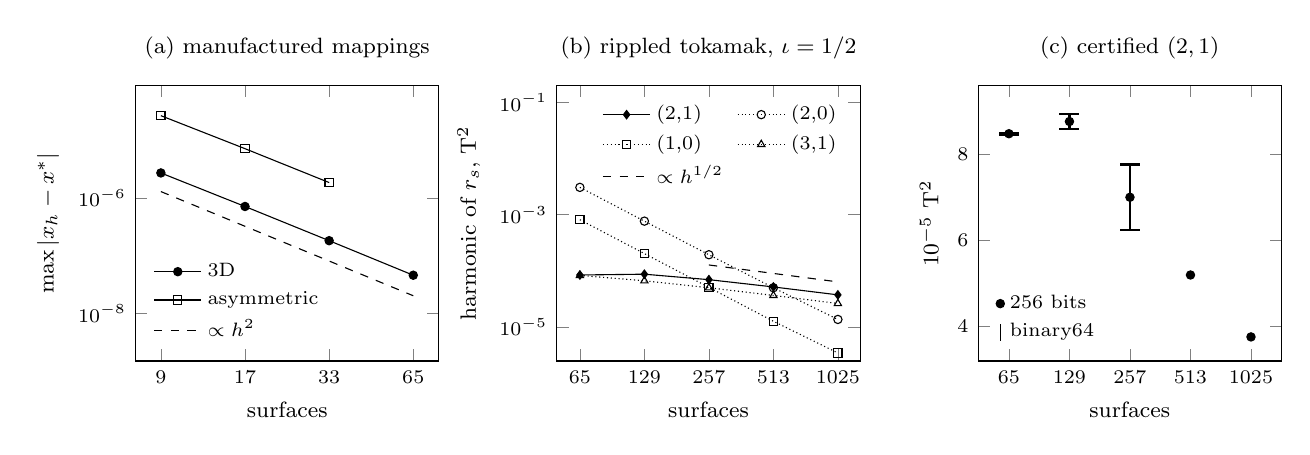
\begin{tikzpicture}
\begin{groupplot}[group style={group size=3 by 1, horizontal sep=1.5cm}, stq]
\nextgroupplot[title={(a) manufactured mappings}, xmode=log, log basis x=2,
  xmin=6.5, xmax=79, xtick={8,16,32,64}, xticklabels={9,17,33,65},
  xlabel={surfaces}, ymode=log, ymin=1.5e-9, ymax=9e-5,
  ylabel={$\max|x_h-x^*|$}, legend pos=south west]
\addplot[mark=*] coordinates {(8,2.73432936829e-6) (16,7.16912170772e-7)
  (32,1.83032585742e-7) (64,4.6074819334e-8)};
\addlegendentry{3D}
\addplot[mark=square] coordinates {(8,2.69073057043e-5) (16,7.20667053290e-6)
  (32,1.86266877703e-6)};
\addlegendentry{asymmetric}
\addplot[dashed, no marks] coordinates {(8,1.3e-6) (64,2.03125e-8)};
\addlegendentry{$\propto h^2$}
\nextgroupplot[title={(b) rippled tokamak, $\iota=1/2$}, xmode=log,
  log basis x=2, xmin=50, xmax=1300, xtick={64,128,256,512,1024},
  xticklabels={65,129,257,513,1025}, xlabel={surfaces}, ymode=log,
  ymin=2.5e-6, ymax=2e-1, ylabel={harmonic of $r_s$, T$^2$},
  legend pos=north east, legend columns=2,
  legend style={/tikz/every even column/.append style={column sep=3pt}}]
\addplot[mark=diamond*] coordinates {(64,8.47827e-5) (128,8.76180e-5)
  (256,7.00294e-5) (512,5.19744e-5) (1024,3.75947e-5)};
\addlegendentry{(2,1)}
\addplot[densely dotted, mark=o] coordinates {(64,3.069800e-3)
  (128,7.699818e-4) (256,1.944837e-4) (512,5.028246e-5) (1024,1.372357e-5)};
\addlegendentry{(2,0)}
\addplot[densely dotted, mark=square] coordinates {(64,8.159535e-4)
  (128,2.038441e-4) (256,5.100695e-5) (512,1.274999e-5) (1024,3.473453e-6)};
\addlegendentry{(1,0)}
\addplot[densely dotted, mark=triangle] coordinates {(64,8.332622e-5)
  (128,6.687446e-5) (256,5.029001e-5) (512,3.672676e-5) (1024,2.638232e-5)};
\addlegendentry{(3,1)}
\addplot[dashed, no marks] coordinates {(256,1.27822e-4) (1024,6.39110e-5)};
\addlegendentry{$\propto h^{1/2}$}
\nextgroupplot[title={(c) certified $(2,1)$}, xmode=log, log basis x=2,
  xmin=45, xmax=1450, xtick={64,128,256,512,1024},
  xticklabels={65,129,257,513,1025}, xlabel={surfaces}, ymin=3.2, ymax=9.6,
  ylabel={$10^{-5}$~T$^2$}, legend pos=south west]
\addplot[only marks, mark=*] coordinates {(64,8.47827) (128,8.76180)
  (256,7.00294) (512,5.19744) (1024,3.75947)};
\addlegendentry{256 bits}
\addlegendimage{only marks, mark=|, mark size=3pt}
\addlegendentry{binary64}
\draw[thick, |-|] (axis cs:64,8.42765) -- (axis cs:64,8.52889);
\draw[thick, |-|] (axis cs:128,8.56369) -- (axis cs:128,8.95991);
\draw[thick, |-|] (axis cs:256,6.21881) -- (axis cs:256,7.78709);
\end{groupplot}
\end{tikzpicture}
\caption{(a) The certified error of the half-grid scheme on the manufactured
mappings; the dashed line falls as $h^2$. (b) Harmonics of the radial force $r_s$
on the surface $\iota=1/2$ of the rippled tokamak: the resonant $(2,1)$ harmonic,
certified at 256 bits (solid), and the floating-point $(2,0)$, $(1,0)$ and
$(3,1)$ harmonics of the same reconstruction (dotted); the dashed line falls as
$h^{1/2}$. (c) The $(2,1)$ harmonic on a linear scale: its binary64 enclosures
at the files' states at 65, 129 and 257 surfaces, and its 256-bit enclosures,
narrower than the dots, at 65 to 1025.}\label{fig:conv}
\end{figure}

\paragraph{A forced current sheet.}
At a rational surface the discrete solution converges more slowly than
anywhere else: the resonant harmonic of the force falls by only 1.2 to 1.4 per
doubling of the surfaces. On VMEC++'s circular tokamak ($R_0=6$, $a=2$) with
$\iota=0.9-0.64s$, which is $1/2$ at $s=0.625$, and a $(1,1)$ boundary ripple of
amplitude $0.03$, toroidal coupling drives a $(2,1)$ harmonic of the radial
force on the rational surface. Its certified value is the rectangle rule for
the integral of $r_s\cos(2u-v)$ on a $64\times32$ grid of angles, in T$^2$ like
$r_s$, against $1.2\times10^3$~T$^2$ for the integral of $B^2$ there. With each
row of the grid evaluated and summed at 256 bits, \code{wdharm\_b\_correct}
encloses it at the states VMEC++ reaches with a tolerance of $10^{-18}$ at 65
to 1025 surfaces, to within a relative $2.1\times10^{-12}$
(Table~\ref{tab:results}, Figure~\ref{fig:conv}c), and it is linear in the
ripple. After a rise of 3.3 per cent from 65 to 129 surfaces it falls by 1.25,
1.35 and 1.38 per doubling, approaching the factor $\sqrt2$ of a decay as
$h^{1/2}$. A decade looser, at $10^{-17}$, the harmonic differs in floating
point by at most 1.3 per cent, and at $10^{-15}$ by up to 6.5 per cent, while
its fall per doubling stays between 1.20 and 1.41 at every tolerance. The axisymmetric harmonics $(2,0)$ and $(1,0)$ of the same
reconstruction fall 3.7 to 4.0-fold per doubling in floating point, and the
$(3,1)$ sideband 1.25 to 1.39-fold (Figure~\ref{fig:conv}b). The same ripple on
a transform profile with no low-order rational surface nearby leaves nothing
behind.

Across the surfaces the harmonic forms a layer. In floating point it peaks
within a radial step of the rational surface and changes sign outside it, and
the distance from its peak to its trough shrinks about as $h^{1/2}$, from 0.117
to 0.040 in $s$ between 129 and 1025 surfaces, while its zero closes on the
rational surface from 0.054 to 0.024. This is the response of a nested-surface field at a
rational surface~\cite{grad1967,hahm1985,loizu2015b}, whose ideal limit is a
current sheet and which~\cite{lazerson2016} studied in VMEC; three-dimensional
equilibria with current sheets and stepped pressure
exist~\cite{bruno1996,enciso2025}. SPEC~\cite{hudson2012} makes the sheet
explicit. With two Beltrami volumes separated by an ideal interface at the
rational surface it is a jump of $1.47\times10^{-5}$ in the covariant poloidal
field at ripple $0.03$, as in the equilibria of~\cite{loizu2015}, and with the
rational surface inside a relaxed volume SPEC's field-line tracing finds a
$(2,1)$ island whose width grows from $0.107$ to $0.173$ in the volume's radial
coordinate as the ripple goes from $0.0075$ to $0.03$, as the ripple to the
power 0.35.

In binary64 interval arithmetic (\code{dharm\_correct}) the harmonic lies
between $5.3\times10^{-5}$ and $9.2\times10^{-5}$ for every state within a
relative $10^{-14}$ of the files' coefficients at 65, 129 and 257 surfaces.
These enclosures widen about fourfold per doubling, from 2.5 to 47 per cent of
the value, as second radial differences amplify a perturbation by $h^{-2}$, and
beyond 257 surfaces a box of that width no longer separates the harmonic from
zero. On the rational surface the
collocated Newton test, its centre refined on outputs read at 128 bits,
certifies a discrete solution at 33 and at 65 surfaces, where the Jacobian's
condition number is $1.4\times10^6$ and $3.0\times10^6$ in floating point.

\paragraph{Free-boundary balance.}
At the free boundary the balance VMEC++ imposes leaves a pressure jump that
radial refinement barely reduces. At a free-boundary equilibrium
$\mu_0p+B^2/2$ is continuous across the plasma boundary, where outside it is the
pressure of the full vacuum field. VMEC++ computes that field with
NESTOR~\cite{merkel1986,hirshman1986}, and BIEST's virtual-casing
field~\cite{malhotra2019,malhotra2020} gives it independently. The certificate
sweeps the vacuum pressure over the segment between the two answers,
$P_{\rm vac}=P_{\rm mid}+t\,\delta P$ with $t\in[-1,1]$, and takes the plasma
side as VMEC's extrapolation of the two outermost half points to $s=1$. The
sweep variable is a slot of the box, which \code{check\_bpcert\_correct} and
\code{check\_btcert\_correct} quantify over separately at each point and in each
cell, so every statement below holds for each vacuum pressure whose value at
each point lies between the two answers there.

On the CTH-like test case, where $B^2/2$ averages $0.18$~T$^2$ on the boundary,
the largest jump on NESTOR's grid is enclosed in $[7.556,7.561]\times10^{-4}$~T$^2$
at 25 surfaces and in $[4.9647,4.9673]\times10^{-4}$~T$^2$ at 385
(Table~\ref{tab:results}, Figure~\ref{fig:equil}a). Each enclosure lies below
the one before it, so the jump does fall, but only by 1.05 to 1.14 per doubling
of the surfaces. The two answers differ by up to $6.1\times10^{-4}$~T$^2$ on the
grid. With the sweep widened to five times that difference the largest jump is
at most $1.89\times10^{-3}$~T$^2$, a hundredth of $B^2/2$, at every resolution.
Covered over the whole boundary by $512\times128$ cells per field period, with
the vacuum side the trigonometric interpolant of each answer's grid, the jump is
at most $8.47\times10^{-3}$~T$^2$ at 25 surfaces and $1.051\times10^{-2}$ at
385. Between grid points that interpolant sets the bound, and radial refinement
leaves its angular resolution as it is.

The jump lies almost wholly beyond the Fourier harmonics through which VMEC
imposes the balance. In floating point at 49 surfaces its part in the retained
harmonics is at most $2.4\times10^{-5}$~T$^2$ and the rest $7.2\times10^{-4}$;
the retained part falls 3.3 and 1.9-fold per doubling from 25 to 97 surfaces,
while with NESTOR's poloidal grid fixed, retaining 5 to 12 poloidal harmonics
moves the jump between $4.0\times10^{-4}$ and $1.5\times10^{-3}$ without
reducing it.

\begin{figure}[t]
\centering
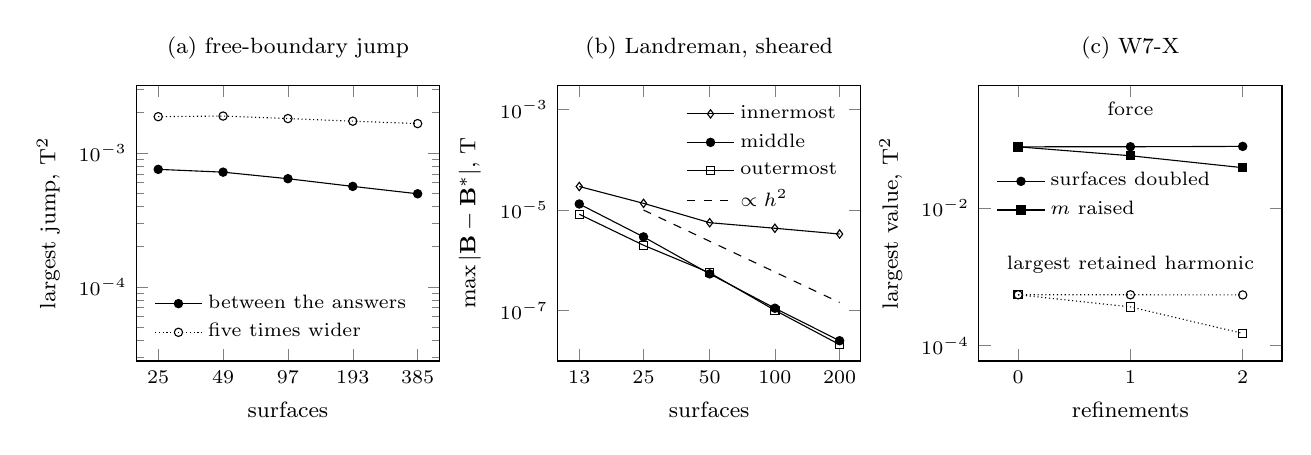
\begin{tikzpicture}
\begin{groupplot}[group style={group size=3 by 1, horizontal sep=1.5cm}, stq]
\nextgroupplot[title={(a) free-boundary jump}, xmode=log, log basis x=2,
  xmin=19, xmax=485, xtick={24,48,96,192,384}, xticklabels={25,49,97,193,385},
  xlabel={surfaces}, ymode=log, ymin=2.8e-5, ymax=3.2e-3,
  ylabel={largest jump, T$^2$}, legend pos=south west]
\addplot[mark=*] coordinates {(24,7.5585e-4) (48,7.2035e-4) (96,6.435e-4)
  (192,5.638e-4) (384,4.966e-4)};
\addlegendentry{between the answers}
\addplot[densely dotted, mark=o] coordinates {(24,1.87e-3) (48,1.89e-3)
  (96,1.81e-3) (192,1.73e-3) (384,1.66e-3)};
\addlegendentry{five times wider}
\nextgroupplot[title={(b) Landreman, sheared}, xmode=log, log basis x=2,
  xmin=9.5, xmax=250, xtick={12,24,49,99,199}, xticklabels={13,25,50,100,200},
  xlabel={surfaces}, ymode=log, ymin=1e-8, ymax=3e-3,
  ylabel={$\max|\mathbf{B}-\mathbf{B}^*|$, T}, legend pos=north east]
\addplot[mark=diamond] coordinates {(12,2.94e-5) (24,1.36e-5) (49,5.61e-6)
  (99,4.35e-6) (199,3.34e-6)};
\addlegendentry{innermost}
\addplot[mark=*] coordinates {(12,1.32e-5) (24,2.93e-6) (49,5.39e-7)
  (99,1.12e-7) (199,2.53e-8)};
\addlegendentry{middle}
\addplot[mark=square] coordinates {(12,8.25e-6) (24,2.00e-6) (49,5.67e-7)
  (99,1.02e-7) (199,2.12e-8)};
\addlegendentry{outermost}
\addplot[dashed, no marks] coordinates {(24,1e-5) (199,1.4545e-7)};
\addlegendentry{$\propto h^2$}
\nextgroupplot[title={(c) W7-X}, xmin=-0.35, xmax=2.35, xtick={0,1,2},
  xlabel={refinements}, ymode=log, ymin=6e-5, ymax=6e-1,
  ylabel={largest value, T$^2$}, legend style={at={(0.03,0.6)}, anchor=west}]
\addlegendimage{mark=*}
\addlegendentry{surfaces doubled}
\addlegendimage{mark=square*}
\addlegendentry{$m$ raised}
\addplot[mark=*, forget plot] coordinates {(0,7.71e-2) (1,7.73e-2) (2,7.82e-2)};
\addplot[mark=square*, forget plot] coordinates {(0,7.71e-2) (1,5.72e-2)
  (2,3.84e-2)};
\addplot[densely dotted, mark=o, forget plot] coordinates {(0,5.49e-4)
  (1,5.49e-4) (2,5.46e-4)};
\addplot[densely dotted, mark=square, forget plot] coordinates {(0,5.49e-4)
  (1,3.66e-4) (2,1.51e-4)};
\node[font=\scriptsize, anchor=south] at (axis cs:1,1.6e-1) {force};
\node[font=\scriptsize, anchor=south] at (axis cs:1,8e-4)
  {largest retained harmonic};
\end{groupplot}
\end{tikzpicture}
\caption{(a) The largest jump of $\mu_0p+B^2/2$ against the vacuum pressure on
NESTOR's grid of the CTH-like case: its certified value for every vacuum
pressure between NESTOR's and BIEST's answers, whose enclosures are narrower than
the dots, and its certified bound for every vacuum pressure within five times
their disagreement. (b) The largest component of $\mathbf{B}-\mathbf{B}^*$
against Landreman's sheared member on the innermost, middle and outermost
half-grid surfaces, certified bounds; the dashed line falls as $h^2$. (c) W7-X:
certified bounds on the largest component of the node residual
$\mu_0(\mathbf{J}\times\mathbf{B}-\nabla p)$ on the surfaces $s=1/4$, $1/2$ and
$3/4$ (filled) and on its largest harmonic at a retained mode (open), as the
surfaces double from 49 to 193 at $m\le11$ and as the angular resolution rises
from $m\le11$ to $m\le19$ at 49 surfaces.}\label{fig:equil}
\end{figure}

\paragraph{The Mercier criterion at coarse resolution.}
At coarse radial resolution the sign of the Mercier criterion depends on how
its radial derivatives are taken, and the certificates prove both signs. At
$s=0.125$ of \code{up\_down\_asym} on 17 surfaces, with 2048 poloidal cells, the
criterion of the Hermite reconstruction is certified unstable: DMerc lies in
$[-1.371,-1.205]\times10^{-3}$ and the current term in
$[-3.724,-3.716]\times10^{-3}$, where the file's own difference quotients give a
stable $+1.8\times10^{-3}$ and a current term of $-6.1\times10^{-4}$.
\code{MercierFile.v} takes the four flux-function derivatives from the file's
centred differences of its half-grid profiles instead, each an exact dyadic,
and integrates the same angular integrands (\code{merc\_run\_q\_correct}): DMerc
then lies in $[1.711,1.875]\times10^{-3}$, which contains the file's value.
The two certified answers differ only in the radial derivatives, so at 17
surfaces those set the sign. From 33 to 257 surfaces both current terms tend to
zero with the file's sign, the certified one from
$[-1.092,-1.083]\times10^{-3}$ to $[-3.7,-1.8]\times10^{-5}$, and the certified
DMerc is positive at each. The equilibrium carries no pressure, so in the
continuum its current and geodesic terms vanish and DMerc reduces to the shear
term, which is never negative: the instability certified at 17 surfaces belongs
to the discretization.

\paragraph{An exact equilibrium.}
Landreman's families~\cite{landreman2026} are three-dimensional equilibria with
nested flux surfaces and smooth field and pressure, which he presents as
counterexamples to Grad's conjecture~\cite{grad1967}. Their field $\mathbf{B}^*$
and flux label $\psi^*$ are elementary functions of the Cartesian position, so a
solver's distance from them is a true error. \code{Landreman.v} and
\code{LandremanSheared.v} prove that both consist of ideal-MHD equilibria: the
family with $\iota=2$ for all positive semiaxes wherever the radicand of
$\mathbf{B}^*$ is positive, and the sheared family for all positive $\epsilon$
and $\lambda$ and every $S$ wherever $(x,y)$ lies off the segment $x=0$,
$|y|\le\sqrt{\epsilon}$. In each the field is solenoidal
(\code{iota2\_divergence}, \code{sheared\_divergence}), satisfies
$(\nabla\times\mathbf{B})\times\mathbf{B}=\nabla p$ with $p=p_a-2\psi$ and
$p=p_a-\psi/\lambda^2$ respectively (\code{iota2\_force},
\code{sheared\_force}), and is tangent to the level sets of $p$
(\code{iota2\_tangent}, \code{sheared\_tangent}). Two outputs of the checker
compare the reconstruction with a member of either family: the cylindrical
components of $\mathbf{B}-\mathbf{B}^*(X)$ on a half-grid surface, with
$\mathbf{B}$ the reconstructed field and $X$ its position, and $\psi^*(X)$ on a
node surface. \code{LandremanExact.v} proves that the expressions behind those
outputs evaluate to the field and flux label of \code{Landreman.v} and of
\code{LandremanSheared.v} on those domains (\code{exact\_b\_iota2},
\code{exact\_b\_sheared}).

Against the sheared family VMEC++'s field converges at about second order away
from the axis. Its solution of the member with $\epsilon=0.6$, $S=2.2$,
$\lambda=2.97$ and $k_b=0.2$, whose transform runs from 4.34 to 4.37, at 13 to
200 surfaces with $m\le11$ and $|n|\le10$, is certified at every point of a
$64\times32$ grid of a field period on its innermost, middle and outermost
half-grid surfaces, where $|\mathbf{B}^*|$ lies between 0.30 and 0.38~T
(Table~\ref{tab:results}, Figure~\ref{fig:equil}b). The radial grids are not
nested, and the middle surface stays near $s=1/2$, at 0.54, 0.52 and then 0.50.
There the certified bound on the largest component of
$\mathbf{B}-\mathbf{B}^*$ falls from $1.32\times10^{-5}$~T at 13 surfaces to
$2.53\times10^{-8}$~T at 200, by 4.4 to 5.4 per doubling. On the outermost
surface it falls from $8.25\times10^{-6}$ to $2.12\times10^{-8}$~T while that
surface moves from $s=0.958$ to $0.997$, toward the fixed boundary, whose
coefficients are the member's own. The innermost surface moves toward the axis,
from $s=0.125$ to $0.008$, and there the bound falls only from
$2.94\times10^{-5}$ to $3.34\times10^{-6}$~T. At the points of the same grid
the outermost node surface, moving from $s=0.917$ to $0.995$, lies within
$2.32\times10^{-7}$ of a level set of $\psi^*$ at 13 surfaces and within
$1.71\times10^{-10}$ at 200, where $\psi^*$ is $0.02$ on the boundary.

Against the member with $\iota=2$, whose every surface is rational, VMEC++'s
field does not converge. Its runs with $m\le9$ and $|n|\le8$ at 13, 25, 50 and
100 surfaces end at their limit of 20000 iterations, their force residual
wandering between $7\times10^{-14}$ and $4\times10^{-10}$ instead of approaching
the tolerance of $10^{-18}$. At one point of the middle half-grid surface a
component of $\mathbf{B}-\mathbf{B}^*$ is at least $7.97\times10^{-4}$,
$2.04\times10^{-4}$, $1.73\times10^{-3}$ and $1.63\times10^{-4}$~T at the four
resolutions, each a floor that \code{check\_bpcert\_correct} proves
(Table~\ref{tab:results}). In floating point 77 to 86 per cent of the
difference's spectral power lies in the resonant harmonics. Those bend no field
line when $\iota=2$ on every surface, so the field-line bending that stiffens
VMEC's energy against every other harmonic does not act on them.

\paragraph{An optimized stellarator.}
On W7-X the certified bound on the force is set by the Fourier truncation and
not by the radial grid. VMEC++'s solution of W7-X from its test data has a volume-averaged
$\beta$ of 4.0 per cent, $m\le11$ and toroidal numbers up to 12 per field
period, and converged to $f_{sqr}<10^{-12}$ at 49, 97 and 193 surfaces. It is
certified at every point of a $64\times64$ grid of a field period on the
surfaces $s=1/4$, $1/2$ and $3/4$ (\code{check\_cert\_correct}), and the same
verdicts enclose the discrete harmonics of each component there at the 288
modes VMEC++ retains (\code{harm\_encloses}). At every resolution the certified
bound on the largest component of the node residual, $\mu_0(\mathbf{J}\times
\mathbf{B}-\nabla p)$ by VMEC's radial differences, is close to
$7.7\times10^{-2}$~T$^2$, and that on its largest harmonic at a retained mode
close to $5.5\times10^{-4}$~T$^2$, at $m=10$, next to the edge of the retained
band (Table~\ref{tab:results}). Raising the angular resolution does what doubling
the surfaces does not: at 49 surfaces with $m\le15$ and $m\le19$, toroidal
numbers up to 16 and 20, the largest component is at most $5.72$ and
$3.84\times10^{-2}$~T$^2$ and the largest retained harmonic at most $3.66$ and
$1.51\times10^{-4}$~T$^2$ (Figure~\ref{fig:equil}c).

\paragraph{Use in VMEC++.}
The certified values are regression tests on a branch of VMEC++~\cite{branch},
whose tolerances are the enclosures: the manufactured-solution errors, the
resonant harmonic with the fall of the axisymmetric harmonics, and the
free-boundary jump, which reads NESTOR's boundary vacuum field through an option
proposed upstream~\cite{pr903}. A finite difference of VMEC++'s energy equals
its unpreconditioned forces contracted with the perturbation, the discrete form
of \code{energy\_gradient\_is\_force}; VMEC++ now tests this~\cite{pr905}, and
that the energy Hessian is symmetric and DGeod never positive~\cite{pr904}. Its
continuous integration now runs VMEC++ on members of both of Landreman's
families on every change and measures, in floating point, its flux surfaces,
magnetic axis, field and enclosed current against the exact
ones~\cite{pr912}.
Differential tests of VMEC++ for invariances the
reconstruction satisfies exactly, three of which VMEC++ now runs~\cite{pr875},
also exposed an orientation test that the poloidal rotation VMEC applies to an
asymmetric boundary can defeat. The test multiplies two $m=1$ coefficients whose
product the rotation can drive to zero, where the invariant is the $m=1$
determinant $r^{cc}z^{sc}-r^{sc}z^{cc}$. Relabelling the
\code{up\_down\_asym\_current} boundary by $\theta\to\pi-\theta$ sends
educational\_VMEC to its iteration cap at $f_{sqr}=2.07\times10^{-2}$ instead of
converging to $5.07\times10^{-12}$. It was reported as
vmecpp\#788~\cite{issue788}, after which VMEC++ tests the
determinant~\cite{pr789}, and as educational\_VMEC\#27~\cite{issue27}.

\section{Consequences for users of VMEC}\label{sec:users}

A converged run does not certify its field. VMEC's normalized force residual
measures the harmonics, at the modes it retains, of the forces the solver
balances, not the force of the field reconstructed from its file. For W7-X
converged to $f_{sqr}<10^{-12}$, the certified bounds on that force at points
of its surfaces and on its largest retained harmonic do not fall as the
surfaces double, while both fall as the poloidal and toroidal resolution rises.
A convergence study of
a stellarator equilibrium therefore has to vary the angular resolution as well
as the number of surfaces, and a quantity computed from the field at points
inherits an error that the angular truncation sets and the residual does not
report. The point and harmonic checks measure that force on any wout file, in
seconds at points and in hours for a harmonic at 256 bits
(Table~\ref{tab:cost}).

Radial convergence away from rational surfaces says little about their
neighbourhood. Near a low-order rational surface the discrete solution forms a
current layer whose resonant force harmonic falls only 1.2 to 1.4-fold per
doubling of the surfaces, so an
equilibrium with such a surface in the plasma converges there far more slowly
than elsewhere. Where every surface is rational, as in Landreman's family with
$\iota=2$, the solution does not converge at all. At coarse radial resolution a
quantity built from radial derivatives of the profiles can change sign with the
way the derivatives are taken: at 17 surfaces the Mercier criterion of
\code{up\_down\_asym} is certified unstable for the reconstruction and stable for
the file's own differences, though without pressure it is stable in the
continuum, and from 33 surfaces on the certified criterion is stable. A Mercier sign near marginal stability from a coarse run should be
confirmed at more surfaces; on a tokamak the certified criterion takes minutes.

At a free boundary the pressure balance barely improves with radial
resolution. The jump of $\mu_0p+B^2/2$ against the vacuum pressure on the
CTH-like boundary falls only from $7.6$ to $5.0\times10^{-4}$~T$^2$, a few
thousandths of $B^2/2$, as the surfaces go from 25 to 385, and retaining more
poloidal harmonics on NESTOR's fixed grid moves it without reducing it.

\section{Related work}

Rigorous numerics proves statements about dynamical systems and partial
differential equations with interval arithmetic: the existence of the Lorenz
attractor~\cite{tucker1999}, the CAPD library for ordinary differential
equations~\cite{capd2021}, KAM theory applied by computer~\cite{figueras2017},
among other systems to magnetic field lines~\cite{valvo2021}, blow-up of the
Boussinesq and axisymmetric Euler equations~\cite{chen2023}, and elliptic and
parabolic problems~\cite{nakao2019}, among them the existence of stationary
Navier--Stokes flows in three-dimensional domains near a computed
approximation~\cite{liu2021}. These proofs run in libraries outside a proof
assistant. Inside one, the closest work is the verified ODE solvers of
Isabelle/HOL up to the Lorenz attractor~\cite{immler2012,immler2018}; the
discretization and floating-point program of the one-dimensional wave
equation~\cite{boldo2013}, the Lax--Milgram theorem~\cite{boldo2017} and
simplicial Lagrange finite elements~\cite{boldo2026} in Rocq, with
floating-point error analysis in VCFloat2 and LAProof~\cite{appel2024,kellison2023};
and the certificates of the Kepler conjecture~\cite{hales2017}. In Lean, high-energy
physics is being formalized~\cite{toobysmith2025}, a formalization has found an
error in the literature on the stability of the two-Higgs-doublet
potential~\cite{toobysmith2026}, the characterization of the equilibria of the
Vlasov--Maxwell--Landau system has been formalized~\cite{ilin2026}, and smooth
magnetohydrostatic equilibria with nested pressure surfaces and only a discrete
rotational symmetry, counterexamples to Grad's conjecture~\cite{grad1967}, come
with a Lean certification~\cite{gomezserrano2026}. In fusion, formal methods
have verified a plasma vertical-position control algorithm~\cite{wu2020} and
properties of neural surrogates of the Grad--Shafranov
equation~\cite{rizqan2025}. Stellarator equilibrium codes are verified by
convergence studies, manufactured solutions and comparison between codes: VMEC
against SPEC~\cite{hudson2012,loizu2015,lazerson2016} and against
DESC~\cite{dudt2020,panici2023}, and against Landreman's explicit
three-dimensional equilibria~\cite{landreman2026}, whose supplement solves them
in DESC. We know of no prior work that states the output of a stellarator
equilibrium code as a machine-checked theorem about the field reconstructed
from it.

\section{Conclusion}

Stellarocq gives the output of an equilibrium code a meaning a proof assistant
can check: bounds, harmonics, Mercier stability terms and the existence of
discrete solutions, each a theorem about the field reconstructed from the
file's exact numbers, whose residual at a free radius is proven to be the
ideal-MHD force. Against Landreman's explicit equilibria~\cite{landreman2026},
both of whose
families the development proves to be ideal-MHD equilibria, the same
certificates measure a solver's error against a true equilibrium and not a
manufactured one.

Floating point gives most of these numbers to several digits; the certificates
add statements of another kind. A verdict is a theorem that rounding cannot
overturn: at 17 surfaces the Mercier criterion is proven negative for the
reconstruction and positive for the file's own differences. A check quantifies
over sets that no finite run samples, every state in a box of coefficients and
every vacuum pressure between the answers of two solvers. It proves what no run
shows, that a discrete solution exists in a given box and that Landreman's
fields are exact equilibria, whose distance from a solver's output is then a
true error. Anyone can check a certificate again with the released checker,
without trusting the program that wrote it.

\paragraph{Limits.}
The certified field is the reconstruction's, and its Hermite extension between
half points is Stellarocq's choice. VMEC's discrete field differs from it by
the products of Section~\ref{sec:object}, whose size on these files is
evaluated in floating point, and the manufactured problems test Stellarocq's
collocation of the half-grid rule, not VMEC's variational equations. A
certificate describes the file it reads, not a converged equilibrium. A small residual does not by itself place an equilibrium nearby, as
fields sustained by a small force show~\cite{constantin2021}. The free-boundary
statements hold for every vacuum pressure between NESTOR's and BIEST's answers,
not for an exact vacuum field, and refine the surfaces with NESTOR's grid
fixed. The Mercier
criterion is certified on the tokamak and not on W7-X, where a covering of
$64\times16$ cells leaves its enclosures unbounded. A check costs seconds at
points and hours for a harmonic at 256 bits or a projection of W7-X at
$m\le19$ (Table~\ref{tab:cost}), and every verdict rests on the trust base of
Section~\ref{sec:certs}.

\paragraph{Availability.}
The development and the certificate generators are at
\link{https://github.com/CharlesCNorton/stellarocq}, where \code{make all}
builds the proofs and the checker and each generator's documentation gives the
commands of its result. Its release \code{v1.0} holds the checker as a static
Linux executable and the certificates behind every certified value of
Sections~\ref{sec:certs} and~\ref{sec:results}, with the VMEC++ files they were
written from, the command that checks each and the verdict it received. The
VMEC++ tests that carry the certified values are on the branch of~\cite{branch}.

\begin{thebibliography}{99}\small\raggedright
\setlength{\itemsep}{1pt}

\bibitem{hirshman1983}
S.~P. Hirshman and J.~C. Whitson, Steepest-descent moment method for
three-dimensional magnetohydrodynamic equilibria, \emph{Phys. Fluids}
\textbf{26}, 3553 (1983).

\bibitem{hirshman1986}
S.~P. Hirshman, W.~I. van~Rij and P.~Merkel, Three-dimensional free boundary
calculations using a spectral Green's function method, \emph{Comput. Phys.
Commun.} \textbf{43}, 143 (1986).

\bibitem{schilling2025}
J.~Schilling, The numerics of VMEC++, arXiv:2502.04374 (2025).

\bibitem{vmecpp}
J.~Schilling, E.~Guiraud and V.~Siska, VMEC++, software,
doi:10.5281/zenodo.14800157.

\bibitem{rocq}
The Rocq Development Team, The Rocq Prover, \link{https://rocq-prover.org}.

\bibitem{letouzey2003}
P.~Letouzey, A new extraction for Coq, in \emph{Types for Proofs and Programs
(TYPES 2002)}, LNCS 2646, 200 (2003).

\bibitem{coquelicot}
S.~Boldo, C.~Lelay and G.~Melquiond, Coquelicot: A user-friendly library of
real analysis for Coq, \emph{Math. Comput. Sci.} \textbf{9}, 41 (2015).

\bibitem{flocq}
S.~Boldo and G.~Melquiond, Flocq: A unified library for proving floating-point
algorithms in Coq, in \emph{20th IEEE Symposium on Computer Arithmetic}, 243
(2011).

\bibitem{melquiond2008}
G.~Melquiond, Proving bounds on real-valued functions with computations, in
\emph{IJCAR 2008}, LNCS 5195, 2 (2008).

\bibitem{mercier1960}
C.~Mercier, A necessary condition for hydromagnetic stability of plasma with
axial symmetry, \emph{Nucl. Fusion} \textbf{1}, 47 (1960).

\bibitem{bauer1984}
F.~Bauer, O.~Betancourt and P.~Garabedian, \emph{Magnetohydrodynamic
Equilibrium and Stability of Stellarators} (Springer, New York, 1984).

\bibitem{krawczyk1969}
R.~Krawczyk, Newton-Algorithmen zur Bestimmung von Nullstellen mit
Fehlerschranken, \emph{Computing} \textbf{4}, 187 (1969).

\bibitem{moore2009}
R.~E. Moore, R.~B. Kearfott and M.~J. Cloud, \emph{Introduction to Interval
Analysis} (SIAM, Philadelphia, 2009).

\bibitem{soloviev1968}
L.~S. Solov'ev, The theory of hydromagnetic stability of toroidal plasma
configurations, \emph{Sov. Phys. JETP} \textbf{26}, 400 (1968).

\bibitem{roache2002}
P.~J. Roache, Code verification by the method of manufactured solutions,
\emph{J. Fluids Eng.} \textbf{124}, 4 (2002).

\bibitem{panici2023}
D.~Panici, R.~Conlin, D.~W. Dudt, K.~Unalmis and E.~Kolemen, The DESC
stellarator code suite. Part 1. Quick and accurate equilibria computations,
\emph{J. Plasma Phys.} \textbf{89}, 955890303 (2023).

\bibitem{grad1967}
H.~Grad, Toroidal containment of a plasma, \emph{Phys. Fluids} \textbf{10}, 137
(1967).

\bibitem{hahm1985}
T.~S. Hahm and R.~M. Kulsrud, Forced magnetic reconnection, \emph{Phys. Fluids}
\textbf{28}, 2412 (1985).

\bibitem{loizu2015b}
J.~Loizu, S.~R. Hudson, A.~Bhattacharjee and P.~Helander, Magnetic islands and
singular currents at rational surfaces in three-dimensional
magnetohydrodynamic equilibria, \emph{Phys. Plasmas} \textbf{22}, 022501
(2015).

\bibitem{lazerson2016}
S.~A. Lazerson, J.~Loizu, S.~Hirshman and S.~R. Hudson, Verification of the
ideal magnetohydrodynamic response at rational surfaces in the VMEC code,
\emph{Phys. Plasmas} \textbf{23}, 012507 (2016).

\bibitem{bruno1996}
O.~P. Bruno and P.~Laurence, Existence of three-dimensional toroidal MHD
equilibria with nonconstant pressure, \emph{Commun. Pure Appl. Math.}
\textbf{49}, 717 (1996).

\bibitem{enciso2025}
A.~Enciso, A.~Luque and D.~Peralta-Salas, MHD equilibria with nonconstant
pressure in nondegenerate toroidal domains, \emph{J. Eur. Math. Soc.}
\textbf{27}, 2251 (2025).

\bibitem{hudson2012}
S.~R. Hudson, R.~L. Dewar, G.~Dennis, M.~J. Hole, M.~McGann, G.~von~Nessi and
S.~Lazerson, Computation of multi-region relaxed magnetohydrodynamic equilibria,
\emph{Phys. Plasmas} \textbf{19}, 112502 (2012).

\bibitem{loizu2015}
J.~Loizu, S.~R. Hudson, A.~Bhattacharjee, S.~Lazerson and P.~Helander,
Existence of three-dimensional ideal-magnetohydrodynamic equilibria with current
sheets, \emph{Phys. Plasmas} \textbf{22}, 090704 (2015).

\bibitem{merkel1986}
P.~Merkel, An integral equation technique for the exterior and interior Neumann
problem in toroidal regions, \emph{J. Comput. Phys.} \textbf{66}, 83 (1986).

\bibitem{malhotra2019}
D.~Malhotra, A.~J. Cerfon, L.-M. Imbert-G\'erard and M.~O'Neil, Taylor states in
stellarators: A fast high-order boundary integral solver, \emph{J. Comput.
Phys.} \textbf{397}, 108791 (2019).

\bibitem{malhotra2020}
D.~Malhotra, A.~J. Cerfon, M.~O'Neil and E.~Toler, Efficient high-order
singular quadrature schemes in magnetic fusion, \emph{Plasma Phys. Control.
Fusion} \textbf{62}, 024004 (2020).

\bibitem{branch}
VMEC++ with Stellarocq's certified values as regression tests, commit
\code{88cdb4cc},
\link{https://github.com/CharlesCNorton/vmecpp/tree/88cdb4cc65fc643e125f5b1440e74792a5ef44a5}.

\bibitem{pr784}
Measure the discretization by the method of manufactured solutions,
\link{https://github.com/proximafusion/vmecpp/pull/784}.

\bibitem{pr903}
Return NESTOR's boundary vacuum field with return\_vacuum\_field,
\link{https://github.com/proximafusion/vmecpp/pull/903}.

\bibitem{pr905}
Test that the unpreconditioned force is the gradient of the MHD energy,
\link{https://github.com/proximafusion/vmecpp/pull/905}.

\bibitem{pr904}
Test that the energy Hessian is symmetric and DGeod is never positive,
\link{https://github.com/proximafusion/vmecpp/pull/904}.

\bibitem{pr912}
Check VMEC++ against exact three-dimensional MHD equilibria in CI,
\link{https://github.com/proximafusion/vmecpp/pull/912}.

\bibitem{pr875}
Test three invariances of the solver,
\link{https://github.com/proximafusion/vmecpp/pull/875}.

\bibitem{issue788}
The Jacobian orientation check is not invariant under the poloidal rotation
applied to an asymmetric boundary, \link{https://github.com/proximafusion/vmecpp/issues/788}.

\bibitem{pr789}
Test the Jacobian orientation with a quantity the lasym rotation preserves,
\link{https://github.com/proximafusion/vmecpp/pull/789}.

\bibitem{issue27}
The Jacobian orientation test is not invariant under the poloidal rotation
applied to an asymmetric boundary,
\link{https://github.com/jonathanschilling/educational\_VMEC/issues/27}.

\bibitem{tucker1999}
W.~Tucker, The Lorenz attractor exists, \emph{C. R. Acad. Sci. Paris S\'er. I
Math.} \textbf{328}, 1197 (1999).

\bibitem{capd2021}
T.~Kapela, M.~Mrozek, D.~Wilczak and P.~Zgliczy\'nski, CAPD::DynSys: a flexible
C++ toolbox for rigorous numerical analysis of dynamical systems,
\emph{Commun. Nonlinear Sci. Numer. Simul.} \textbf{101}, 105578 (2021).

\bibitem{figueras2017}
J.-Ll.~Figueras, A.~Haro and A.~Luque, Rigorous computer-assisted application
of KAM theory: a modern approach, \emph{Found. Comput. Math.} \textbf{17}, 1123
(2017).

\bibitem{valvo2021}
L.~Valvo and U.~Locatelli, Hamiltonian control of magnetic field lines:
computer assisted results proving the existence of KAM barriers, \emph{J.
Comput. Dyn.} \textbf{9}, 505 (2022).

\bibitem{chen2023}
J.~Chen and T.~Y. Hou, Stable nearly self-similar blowup of the 2D Boussinesq
and 3D Euler equations with smooth data II: Rigorous numerics, \emph{Multiscale
Model. Simul.} \textbf{23}, 25 (2025).

\bibitem{nakao2019}
M.~T. Nakao, M.~Plum and Y.~Watanabe, \emph{Numerical Verification Methods and
Computer-Assisted Proofs for Partial Differential Equations} (Springer,
Singapore, 2019).

\bibitem{liu2021}
X.~Liu, M.~T. Nakao and S.~Oishi, Computer-assisted proof for the stationary
solution existence of the Navier--Stokes equation over 3D domains, \emph{Commun.
Nonlinear Sci. Numer. Simul.} \textbf{108}, 106223 (2022).

\bibitem{immler2012}
F.~Immler and J.~H\"olzl, Numerical analysis of ordinary differential equations
in Isabelle/HOL, in \emph{Interactive Theorem Proving (ITP 2012)}, LNCS 7406,
377 (2012).

\bibitem{immler2018}
F.~Immler, A verified ODE solver and the Lorenz attractor, \emph{J. Autom.
Reason.} \textbf{61}, 73 (2018).

\bibitem{boldo2013}
S.~Boldo, F.~Cl\'ement, J.-C. Filli\^atre, M.~Mayero, G.~Melquiond and P.~Weis,
Wave equation numerical resolution: A comprehensive mechanized proof of a C
program, \emph{J. Autom. Reason.} \textbf{50}, 423 (2013).

\bibitem{boldo2017}
S.~Boldo, F.~Cl\'ement, F.~Faissole, V.~Martin and M.~Mayero, A Coq formal proof
of the Lax--Milgram theorem, in \emph{6th ACM SIGPLAN Conference on Certified
Programs and Proofs (CPP 2017)}, 79 (2017).

\bibitem{boldo2026}
S.~Boldo, F.~Cl\'ement, V.~Martin, M.~Mayero and H.~Mouhcine, A Rocq
formalization of simplicial Lagrange finite elements, arXiv:2604.20345 (2026).

\bibitem{appel2024}
A.~W. Appel and A.~E. Kellison, VCFloat2: Floating-point error analysis in Coq,
in \emph{CPP 2024} (2024).

\bibitem{kellison2023}
A.~E. Kellison, A.~W. Appel, M.~Tekriwal and D.~Bindel, LAProof: A library of
formal proofs of accuracy and correctness for linear algebra programs, in
\emph{ARITH 2023} (2023).

\bibitem{hales2017}
T.~Hales et al., A formal proof of the Kepler conjecture, \emph{Forum Math. Pi}
\textbf{5}, e2 (2017).

\bibitem{toobysmith2025}
J.~Tooby-Smith, HepLean: Digitalising high energy physics, \emph{Comput. Phys.
Commun.} \textbf{308}, 109457 (2025).

\bibitem{toobysmith2026}
J.~Tooby-Smith, Formalizing the stability of the two Higgs doublet model
potential into Lean: identifying an error in the literature, arXiv:2603.08139
(2026).

\bibitem{ilin2026}
V.~Ilin, Semi-autonomous formalization of the Vlasov--Maxwell--Landau
equilibrium, arXiv:2603.15929 (2026).

\bibitem{gomezserrano2026}
J.~G\'omez-Serrano, L.~Liehr and M.~A. Taylor, Counterexamples to Grad's
conjecture, arXiv:2609.24739 (2026).

\bibitem{wu2020}
M.~Wu, J.~Rosenberg and N.~Fulton, A formally verified plasma vertical position
control algorithm, in \emph{Formal Methods for Industrial Critical Systems
(FMICS 2020)}, LNCS 12327, 170 (2020).

\bibitem{rizqan2025}
F.~N. Rizqan, M.~Hole and C.~Gretton, Evaluation and verification of
physics-informed neural models of the Grad--Shafranov equation,
arXiv:2504.21155 (2025).

\bibitem{dudt2020}
D.~W. Dudt and E.~Kolemen, DESC: A stellarator equilibrium solver, \emph{Phys.
Plasmas} \textbf{27}, 102513 (2020).

\bibitem{landreman2026}
M.~Landreman, Analytic toroidal 3D MHD equilibria and steady Euler flows with
invariant surfaces, arXiv:2609.26742 (2026).

\bibitem{constantin2021}
P.~Constantin, T.~D. Drivas and D.~Ginsberg, On quasisymmetric plasma
equilibria sustained by small force, \emph{J. Plasma Phys.} \textbf{87},
905870111 (2021).

\end{thebibliography}

\end{document}
